\documentclass[10pt,twocolumn]{article}

\usepackage[T1]{fontenc}
\usepackage[utf8]{inputenc}
\usepackage{lmodern}
\usepackage[a4paper,margin=0.5in,columnsep=0.22in]{geometry}
\usepackage{amsmath}
\usepackage{booktabs}
\usepackage{tabularx}
\usepackage{array}
\usepackage{graphicx}
\usepackage{caption}
\usepackage[shortlabels]{enumitem}
\usepackage{microtype}
\usepackage{titlesec}
\usepackage[hidelinks]{hyperref}

\titleformat*{\section}{\large\bfseries}
\titlespacing*{\section}{0pt}{6pt}{3pt}
\titlespacing*{\paragraph}{0pt}{3pt}{0.5em}
\raggedbottom
\setlength{\textfloatsep}{6pt}
\setlength{\abovecaptionskip}{3pt}
\setlength{\belowcaptionskip}{0pt}
\setlist{nosep,leftmargin=*}
\setlength{\parskip}{0pt}
\newcolumntype{Y}{>{\raggedright\arraybackslash}X}
\newcommand{\ci}[2]{[$#1$, $#2$]}

\title{\vspace{-0.4in}Confidence-Based Query Routing for Hybrid Retrieval: Final Report}
\author{\normalsize
  G Sai Sri Harsha (2024101034), Parth Shashank Dhodapkar (2024111009), Joshua Athelstan Koilpillai (2024101128)\\
  \normalsize\textbf{Team:} Ching's Sonion Rings \quad
  \textbf{Presentation:} \href{https://drive.google.com/drive/folders/1VuHwiwowSJQMIVN0N5-4-laXq_mDwFmC?usp=sharing}{Google Drive folder} \quad
  \textbf{GitHub:} \href{https://github.com/thereal-slimshady123/ire_project}{thereal-slimshady123/ire\_project}%
}
\date{\vspace{-0.3in}}

\begin{document}
\maketitle

\noindent\textbf{Abstract.} We tested whether a cheap per-query router can choose between BM25, dense and hybrid retrieval, and send uncertain queries to a cross-encoder, better than a single tuned hybrid. On held-out queries it cannot: the pre-registered router is $0.0073$ nDCG@10 below always-hybrid, and the full system with budgeted escalation is $0.0053$ below. Pre-registered follow-up tests on 16 further datasets show why. No group of queries identifiable before retrieval prefers one retriever, and which retriever wins depends mostly on the relevant document, not the query. A per-document fusion model gives a small gain over hybrid ($+0.0029$ \ci{+0.0019}{+0.0038}). Skipping dense retrieval for about a third of queries costs little quality, but saves time only on some corpora.

\section{Problem}

Search systems usually combine BM25, which matches exact words, with a dense (embedding) retriever, which matches meaning. A hybrid mixes their scores with one fixed weight $\alpha$. A cross-encoder can then re-rank the top results, but it is slow. We asked whether a cheap per-query decision could beat one fixed hybrid: (1)~pick BM25, dense or hybrid for each query from features of the query and the first results; (2)~send only uncertain queries to the cross-encoder, within a small budget. We expected better ranking at similar cost. Held-out results do not support this: always-hybrid is the best cheap policy. Phase~2 explains why, and finds a small gain from a different approach.

\paragraph{Prior work and what is new.} Arabzadeh, Yan and Clarke (CIKM 2021) already predict per query whether to use sparse, dense or hybrid retrieval, so per-query routing itself is not new. We add held-out evaluation against a tuned hybrid with matched random controls, budgeted cross-encoder escalation, and a split-half test of why routing fails. Learning-to-rank fusion (our E6 model) is a known technique; our contribution is the evidence that it beats routing.

\section{Setup}

\begin{itemize}
  \item \textbf{Retrievers:} BM25 ($k_1{=}1.2$, $b{=}0.75$), dense \texttt{intfloat/e5-small-v2}, hybrid with $\alpha$ tuned on training folds, RRF as a baseline. Top-100 lists.
  \item \textbf{Features:} 18 per query (6 about the query text, 12 about the retrieval results: score gaps, list overlap, rank correlation and so on).
  \item \textbf{Evaluation:} nDCG@10; 5-fold cross-validation by query (seed 42); paired bootstrap, 10,000 resamples; practical margin $\delta = 0.005$. All results are on held-out queries.
  \item \textbf{Phase 1 data:} NFCorpus, SciFact, FiQA, CQADupStack-Unix and a Quora subset (3,343 queries).
  \item \textbf{Phase 2 data:} \emph{exploration} data (19 already-seen datasets) formed the hypotheses and, for 16 of them, trained the E6 model. \emph{Held-out} data (16 datasets: validation, fresh, boundary and Climate-FEVER sets) was used once each for the pre-registered tests, covering forums, science, open-domain and multi-hop QA, entity search and fact-checking. A second encoder (e5-base) was used for robustness.
\end{itemize}

\begin{table*}[t]
\centering
\caption{Phase 2 pre-registered hypotheses and verdicts.}
\label{tab:p2}
\begin{tabularx}{\textwidth}{@{}l>{\raggedright\arraybackslash}p{0.36\textwidth}Y@{}}
\toprule
 & Hypothesis & Verdict \\
\midrule
E1 & A router trained on synthetic queries fails on real ones & \textbf{Accepted.} $-0.0209$ \ci{-0.0256}{-0.0162} vs hybrid. Length alone predicts synthetic winners perfectly; best real feature AUC$'$ 0.60. \\
E2 & No pre-retrieval query group does better with one retriever & \textbf{Accepted in four tests.} BM25 and dense below hybrid in every group; router within $\pm 0.002$; best AUC$'$ 0.57--0.60. \\
E3/E3$'$ & A skip router avoids dense retrieval for $\ge$20\% of queries & Not met / inconclusive, both as predicted (12--13\% skipped on forums). \\
E4 & The winner is a property of the document, not the query & \textbf{Inconclusive.} Pooled AUC$'$ 0.7498 (reject at 0.75), driven by HotpotQA; 0.522 without it. \\
E4-R & E4 redone on Climate-FEVER & \textbf{Accepted.} AUC$'$ 0.507, which is chance. \\
E5 & A small frozen niche where routing wins & \textbf{Rejected}, as predicted. \\
E6 & Fusing per document beats fixed-$\alpha$ hybrid & \textbf{Accepted.} $+0.0029$ \ci{+0.0019}{+0.0038} pooled. \\
E7 & The free BM25-ratio rule matches the learned skip router & Inconclusive (5 of 6 datasets, not HotpotQA). \\
E8 & Multi-hop data is the exception & Inconclusive. 2WikiMultihopQA behaves like HotpotQA; MuSiQue does not. \\
\bottomrule
\end{tabularx}
\end{table*}

\section{Phase 1: Does routing work?}

\noindent\begin{tabularx}{\columnwidth}{@{}l>{\raggedright\arraybackslash}p{0.27\columnwidth}Y@{}}
\toprule
 & Hypothesis & Result \\
\midrule
H1 & Beats hybrid and RRF & \textbf{Not supported.} GBM router $-0.0073$ \ci{-0.0100}{-0.0045} vs hybrid. The cost-aware router beats RRF ($+0.0142$), but so does plain hybrid ($+0.0153$). \\
H2 & Recall@100 level with hybrid & \textbf{Supported.} GBM, cost-aware and router${}+\tau$ within $\pm 0.01$; the logistic router is not ($-0.0224$). \\
H3 & 10\% escalation keeps most rerank gain & \textbf{Not supported.} The plain reranker is worse than hybrid. With a blended score, a 10\% budget keeps 16\% of the gain. \\
H4 & Latency near hybrid & \textbf{Partly.} Router adds 5--13\,ms; 10\% escalation costs 1.2--7$\times$ hybrid; always-rerank 348--406\,ms/query (45\,ms on Quora). \\
\bottomrule
\end{tabularx}

\begin{itemize}
  \item \textbf{Headroom is small and mostly noise.} A per-query oracle beats hybrid by $+0.034$, but an ``oracle'' over three near-identical hybrids already gets $+0.015$. The real headroom is about $+0.02$, and no held-out router reaches it.
  \item \textbf{Class balancing caused much of the loss.} A cost-aware router (no balancing, falls back to hybrid unless inner CV shows a gain) reaches $-0.0012$ \ci{-0.0025}{+0.0002}: not worse than hybrid, but not better.
  \item \textbf{Dual advantage regression} (predicts each retriever's gain over hybrid, routes only past a risk threshold, with a $z \ge 1.645$ guard) sends 99\% of queries to hybrid: $-0.0001$ \ci{-0.0007}{+0.0003}. With fixed thresholds and no guard: $-0.0009$ \ci{-0.0028}{+0.0009}. Every feature subset stays within $\pm 0.0003$ of hybrid; the classifier is significantly below hybrid for every subset.
  \item \textbf{Rerankers.} MiniLM-L6, MiniLM-L12 and BGE-base all lower nDCG@10 on these pools. Blending the cross-encoder score with the hybrid score beats hybrid ($+0.0067$ \ci{+0.0035}{+0.0098} on every query). Reranking only each query's top-20 keeps the full gain at about 40\% of the cost (post hoc).
  \item \textbf{Router${}+\tau$ escalation} (the proposal's full system): escalates when the router's top probability falls below $\tau$. At a 10\% target (9.5\% realized): $-0.0053$ \ci{-0.0088}{-0.0019} vs hybrid, $+0.0026$ \ci{+0.0003}{+0.0050} vs random escalation. Router confidence picks out the router's own mistakes (risk-coverage beats random on all five datasets) but not where reranking helps.
  \item \textbf{Skipping dense retrieval is the one pre-registered success (Exp.~3).} 32.9\% of queries skipped at $-0.0053$ vs hybrid, $+0.0104$ vs random skipping. A free BM25 top-1/top-2 score-ratio rule does as well. Latency changes from $-40\%$ (Quora) to $+20\%$ (FiQA).
\end{itemize}

\begin{figure}[t]
  \centering
  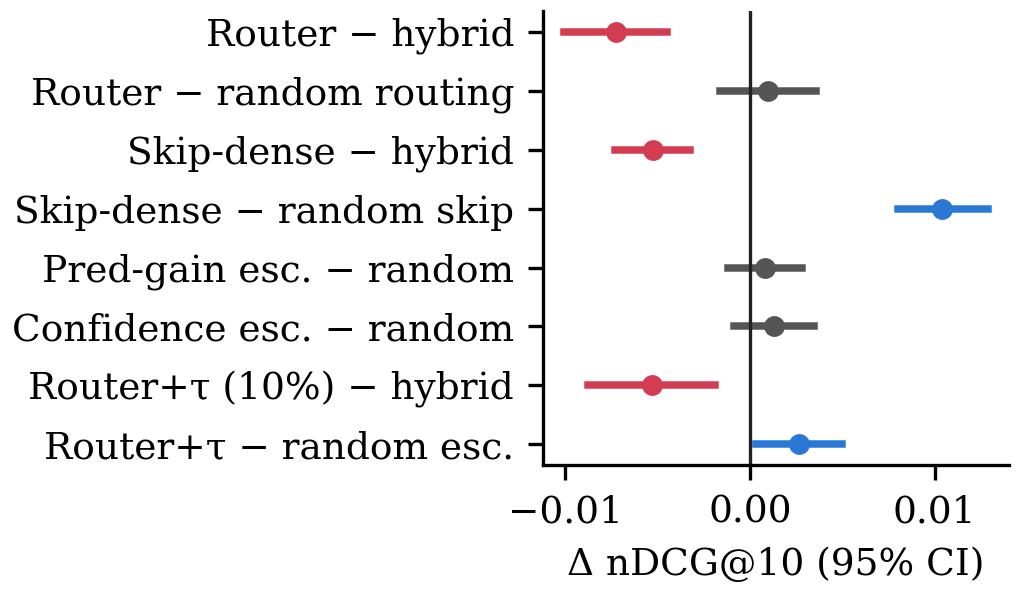
\includegraphics[width=\columnwidth]{figures/comparisons_forest_column.png}
  \caption{Pooled paired differences in nDCG@10 with 95\% bootstrap CIs. Routing, with or without $\tau$ escalation, is below always-hybrid; dense skipping and router${}+\tau$ escalation beat their random controls.}
\end{figure}

\section{Phase 2: Why does routing fail?}

Each hypothesis was pre-registered (written and hashed before its data was downloaded) and run once on held-out datasets chosen by fixed rules (Table~\ref{tab:p2}).

\paragraph{Main finding (E4/E4-R).} We split each query's relevant documents in half and checked whether the same retriever wins both halves. It mostly does not (AUC$'$ near 0.5), so there is little for a query-level router to learn. Multi-hop datasets, where all relevant documents are needed together, are the exception.

\paragraph{What works instead (E6).} A LightGBM LambdaRank model scores each candidate document from normalised BM25 and dense scores, ranks and the query features. Trained once on 16 exploration datasets and applied unchanged to six fresh ones, it gains $+0.0029$ over hybrid, positive on all six and significant on two (NQ, HotpotQA), for about 5\,ms more per query. Against an $\alpha$ tuned on each target's own labels the gain is $+0.0011$ \ci{+0.0000}{+0.0021}, and NQ is significantly worse. The effect is small.

\paragraph{Checks that the null result is real.} Removing the router's hybrid fallback makes it worse ($-0.0023$), so the fallback is a symptom, not the cause. Weighting every query group equally (macro nDCG) leaves the router within $\pm 0.0011$ of hybrid, with BM25 or dense alone 0.03--0.09 below it. 9 of 13 pre-registered predictions were correct. All four misses involve multi-hop data.

\section{Conclusions}

\begin{enumerate}
  \item Always-hybrid is the strongest dependable cheap policy. No router or selective-escalation policy beats it on natural queries.
  \item Routing fails because the right retriever is largely decided per document, not per query, and pre-retrieval features cannot see that.
  \item Synthetic query sets make routing look like it works, an artefact of how they are built.
  \item Skipping dense retrieval is feasible for about a third of queries at a small quality cost, and a free score-ratio rule does as well as a learned model. It saves time only when the corpus or encoder is expensive enough.
  \item Per-document fusion gives a small gain ($+0.003$) at small cost. Blended reranking also beats hybrid ($+0.0067$) but at 40\% or more of full-rerank cost, so per-document fusion is the only cheap gain.
\end{enumerate}

\section{Limitations}

\begin{itemize}
  \item All effects are small, and per-dataset sample sizes are modest. One encoder family (e5), one fusion form (min-max convex), one candidate depth. Latency was measured on one laptop, one pass per query.
  \item Large corpora were capped at 50,000 documents, which makes retrieval easier than on the full collections.
  \item The split-half test covers only queries with at least two relevant documents. Climate-FEVER's judgments may be noisy, which alone would push its AUC$'$ towards 0.5.
  \item The e5 encoder was trained on data that includes NQ, so NQ is not new to it. E4's pooled design was a mistake, corrected afterwards in E4-R. Both are reported.
\end{itemize}

\end{document}
